\documentclass{beamer}

\usepackage{graphicx}
\usepackage{float}
\usepackage{xcolor}

% Colors of baseline agents
\definecolor{color_base0}{RGB}{203, 4, 2}
\definecolor{color_base1}{RGB}{188, 28, 98}
\definecolor{color_base2}{RGB}{163, 5, 245}
\definecolor{color_base3}{RGB}{83, 21, 182}

%Information to be included in the title page:
\title{Energy Efficiency in Railway Scheduling}
\author{Paul Tennigkeit, Georgi Abshilava}
\institute{Universität Potsdam}
\date{21.09.2026}

\begin{document}

\frame{\titlepage}

\begin{frame}
\frametitle{Outline}
\tableofcontents
\end{frame}

\section{Motivation: Energy Efficiency Problem}
\begin{frame}
\frametitle{Motivation: Energy Efficiency Problem}

\end{frame}

\section{Baseline ASP Model}
\begin{frame}
\frametitle{Baseline ASP Model}
\begin{itemize}
  \item Establishes rules to handle essential train behavior
  \begin{itemize}
    \item Directions
    \item Movements
    \item Transitions
    \item Collision and Reachability Constraints
    \item Schedule Optimization
  \end{itemize}
\end{itemize}
\end{frame}

\begin{frame}[fragile]
\frametitle{Directions and Movements}
  \begin{verbatim}
% Directions
dir(s).
dir(n).
dir(w).
dir(e).
  
% Movement Operation
moving(move_forward).
moving(move_left).
moving(move_right).
  
% Movement on Grid
delta(A,s,1,0)  :- moving(A).
delta(A,n,-1,0) :- moving(A).
delta(A,e,0,1)  :- moving(A).
delta(A,w,0,-1) :- moving(A).
  \end{verbatim}
\end{frame}

\begin{frame}[fragile]
\frametitle{Transitions}
  \begin{verbatim}
% Transition facts: To represent different track types
% ID : track ID
% Dir1: pointing direction of agent
% Act : associated action with movement towards exit
% Dir2: exit direction
transition(ID, Dir1, Act, Dir2).
  \end{verbatim}
\end{frame}

\begin{frame}[fragile]
\frametitle{Collision Constraints}
  \begin{verbatim}
% Trains can not occupy the same cell at the same time
:- stay(ID1,X,Y,T),
   stay(ID2,X,Y,T),
   ID1 < ID2.

% Trains can not swap their position
:- stay(ID1,X1,Y1,T),
   stay(ID2,X2,Y2,T),
   stay(ID1,X2,Y2,T+1),
   stay(ID2,X1,Y1,T+1),
   ID1 < ID2.
  \end{verbatim}
\end{frame}

\begin{frame}[fragile]
\frametitle{Reachability Constraints}
  \begin{verbatim}
% define states (cell, time, direction),
% which are reachable by a train 
reachable(ID,T,A,X2,Y2,T2,Dir2) :-
                            A != wait,
                            position(ID,(X,Y),T,Dir1),
                            cell((X,Y),Cell),
                            transition(Cell,Dir1,A,Dir2),
                            delta(A,Dir2,DX,DY),
                            X2 = X + DX,
                            Y2 = Y + DY,
                            speed(ID,S),
                            T2 = T + S,
                            time(T2).
reachable(ID,T,wait,X,Y,T+1,Dir) :-
                            position(ID,(X,Y),T,Dir),
                            time(T+1).
  \end{verbatim}
\end{frame}

\begin{frame}[fragile]
\frametitle{Reachability Constraints}
  \begin{verbatim}
% Choose exactly one valid transition at each time step
1 { position(ID,(X2,Y2),T2,Dir2)
    : reachable(ID,T,A,X2,Y2,T2,Dir2)
} 1 :- position(ID,(_,_),T,_),
       not reached(ID,T).
       
% Track the time interval a train spends inside a cell.
% This is to make enforcing collision constraints easier.
chosen(ID,T,A,X,Y,X2,Y2,T2) :-
                       position(ID,(X,Y),T,_),
                       position(ID,(X2,Y2),T2,_),
                       reachable(ID,T,A,X2,Y2,T2,_).
                       
% a train reached its target if their position matches 
reached(ID,T) :- position(ID,(X,Y),T,_),
                 end(ID,(X,Y),_).
  \end{verbatim}
\end{frame}

\begin{frame}[fragile]
\frametitle{Schedule Optimization}
\begin{verbatim}
% stop searching if train is not
% in time to reach its target anymore
:- position(ID,(X,Y),T,_),
   end(ID,(EX,EY),Arr),
   speed(ID,InvSpd),
   T + (|X-EX| + |Y-EY|)*InvSpd > Arr.
   
% the arrival times should be minimized
reached_earlier(ID,T) :- reached(ID,T),
                         reached(ID,T0), T0 < T.
arrival(ID,T) :- reached(ID,T),
                 not reached_earlier(ID,T).

% minimize summed arrival times
#minimize { T@2,ID : arrival(ID,T) }.
\end{verbatim}
\end{frame}

\begin{frame}
\begin{figure}[H]
  \centering
  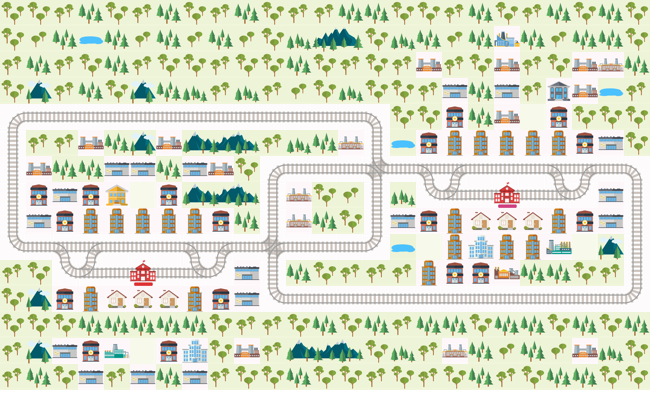
\includegraphics[width=0.6\textwidth]{images/environment.png}
  \caption{Environment used to test the encodings}
  \label{fig:environment_image}
\end{figure}
\end{frame}

\begin{frame}
\begin{table}
\centering
%\scriptsize
\caption{Train 0}
\label{tab:base0}
\begin{tabular}{c c c c c}
\hline
\textbf{Time step} & \textbf{Position} & \textbf{direction} & \textbf{status} & \textbf{Given Command} \\
\hline
34 & (11, 1) & s & moving & move\_forward \\
35 & (12, 1) & s & moving & move\_forward \\
36 & (13, 1) & s & moving & move\_forward \\
37 & (13, 2) & e & moving & move\_forward \\
38 & (13, 3) & e & moving & move\_forward \\
39 & (13, 4) & e & moving & move\_forward \\
40 & (13, 5) & e & moving & move\_forward \\
\hline
\end{tabular}
\end{table}
\end{frame}

\begin{frame}
\begin{table}
\centering
%\scriptsize
\caption{Train 1}
\label{tab:base1}
\begin{tabular}{c c c c c}
\hline
\textbf{Time step} & \textbf{Position} & \textbf{direction} & \textbf{status} & \textbf{Given Command} \\
\hline
34 & (7, 20) & w & moving & move\_forward \\
35 & (7, 19) & w & moving & move\_forward \\
36 & (7, 18) & w & moving & move\_forward \\
37 & (7, 17) & w & moving & move\_forward \\
38 & (7, 16) & w & moving & move\_forward \\
39 & (7, 15) & w & moving & move\_forward \\
40 & (7, 14) & w & moving & move\_forward \\
\hline
\end{tabular}
\end{table}
\end{frame}

\section{Acceleration Mechanics}
\begin{frame}
\frametitle{Acceleration Mechanics}
\begin{itemize}
  \item Speed Changes in General
  \item Turning, Waiting, and Arrival Physics
  \item Solver Heuristics
\end{itemize}
\end{frame}

\begin{frame}[fragile]
\frametitle{Speed Changes in General}
\begin{verbatim}
% Interpret given train speeds as maximum speeds
max_speed(ID,S) :- speed(ID,S).

% Trains start with a speed of 1/4 
temp_speed(ID, Dep+1, 4) :- start(ID,(_,_),Dep,_).
\end{verbatim}
\end{frame}

\begin{frame}[fragile]
\frametitle{Speed Changes in General}
\begin{verbatim}
% Allow gradual speed changed, while
% respecting the physical limits of the train.
% The train can change its speed up to one
% step at a time
1{
  temp_speed(ID,T2,S-1);
  temp_speed(ID,T2,S);
  temp_speed(ID,T2,S+1)
}1 
:- chosen(ID,T,A,_,_,_,_,T2),
   A != wait,
   temp_speed(ID,T,S),
   max_speed(ID,MS),
   S-1 >= MS,
   S+1 <= 4.

\end{verbatim}
\end{frame}

\begin{frame}[fragile]
\frametitle{Speed Changes in General}
\begin{verbatim}
% Lower Bound
1{
  temp_speed(ID,T2,S-1);
  temp_speed(ID,T2,S)
}1
:- chosen(ID,T,A,_,_,_,_,T2),
   A != wait,
   temp_speed(ID,T,S),
   max_speed(ID,MS),
   S-1 >= MS,
   S+1 > 4.
\end{verbatim}
\end{frame}

\begin{frame}[fragile]
\frametitle{Speed Changes in General}
\begin{verbatim}
% Upper Bound
1{
  temp_speed(ID,T2,S);
  temp_speed(ID,T2,S+1)
}1
:- chosen(ID,T,A,_,_,_,_,T2),
   A != wait,
   temp_speed(ID,T,S),
   max_speed(ID,MS),
   S-1 < MS,
   S+1 <= 4.
\end{verbatim}
\end{frame}

\begin{frame}[fragile]
\frametitle{Speed Changes in General}
\begin{verbatim}
% In between (maintain speed)
temp_speed(ID,T2,S) :- chosen(ID,T,A,_,_,_,_,T2),
                       A != wait,
                       temp_speed(ID,T,S),
                       max_speed(ID,MS),
                       S-1 < MS,
                       S+1 > 4.
\end{verbatim}
\end{frame}

\begin{frame}[fragile]
\frametitle{Turning, Waiting, and Arrival Physics}
\begin{verbatim}
% You have to take a turn with inverse speed >= 3 
:- position(ID,_,T,Dir1),
   temp_speed(ID,T,S),
   T2 = T + S,
   position(ID,_,T2,Dir2),
   Dir1 != Dir2,
   S < 3.
\end{verbatim}
\end{frame}

\begin{frame}[fragile]
\frametitle{Turning, Waiting, and Arrival Physics}
\begin{verbatim}
% to be able to wait, you need to have speed 1/4
reachable(ID,T,wait,X,Y,T+1,Dir) :- 
                            position(ID,(X,Y),T,Dir),
                            time(T+1),
                            temp_speed(ID,T,4).

% after waiting, you have to start with speed 1/4
temp_speed(ID,T2,4) :- chosen(ID,T,wait,_,_,_,_,T2).
\end{verbatim}
\end{frame}

\begin{frame}[fragile]
\frametitle{Turning, Waiting, and Arrival Physics}
\begin{verbatim}
% you can only arrive at your goal if your 
% inverse speed was 4 before
:- reached(ID,T2),
   temp_speed(ID,T1,S),
   T2 = T1 + S,
   S < 4.
\end{verbatim}
\end{frame}

\begin{frame}[fragile]
\frametitle{Solver Heuristics}
\begin{verbatim}
% prefer to not wait
wait_position(ID,X2,Y2,T2,Dir2) :-
                     reachable(ID,T,wait,X2,Y2,T2,Dir2).
                     
#heuristic position(ID,(X2,Y2),T2,Dir2)
           : wait_position(ID,X2,Y2,T2,Dir2).
           [-50,1]

% schedule trains one by one
#heuristic position(ID,(X,Y),T,Dir) : start(ID,_,Dep,_).
           [-Dep,1]

% prefer getting faster
#heuristic temp_speed(ID,T,S) : position(ID,_,T,_).
           [-S,1]
\end{verbatim}
\end{frame}

\section{Energy Mechanics}
\begin{frame}
\frametitle{Energy Mechanics}
\begin{itemize}
  \item Energy Cost Factors and Power Types
  \item Energy Consumption for Different Types of Actions (Braking, Turning, Coasting)
  \item Encoding Optimization
\end{itemize}
\end{frame}

\begin{frame}[fragile]
\frametitle{Cost Factors and Power Types}
\begin{verbatim}
% Energy cost factor of trains
% based on power type + weight
pow_cost_fac(ID,1) :- pow_type(ID, electro).
pow_cost_fac(ID,2) :- pow_type(ID, hybrid).
pow_cost_fac(ID,3) :- pow_type(ID, diesel).
pow_cost_fac(ID,4) :- pow_type(ID, hydrogen).

% A train's weight is defined in
% the environment's logic program
cost_fac(ID,CF) :- pow_cost_fac(ID,PCF),
                   weight(ID,W),
                   CF = PCF * W.
\end{verbatim}
\end{frame}

\begin{frame}[fragile]
\frametitle{Cost of Braking}
\begin{verbatim}
% Tracks whether the train was waiting
% in the previous time step
prev_wait(ID,T) :- action(train(ID),_,T),
                   time(T-1),
                   action(train(ID),wait,T-1).

energy(ID,T+1,E) :- action(train(ID),wait,T),
                    speed(ID,S),
                    not prev_wait(ID,T),
                    cost_fac(ID,CF),
                    E = CF * 24 / S.
\end{verbatim}
\end{frame}

\begin{frame}[fragile]
\frametitle{Cost of Coasting}
\begin{verbatim}
energy(ID,T2,E) :- action(train(ID),A,T),
                   A != wait,
                   position(ID,_,T,Dir),
                   speed(ID,S),
                   T2 = T + S,
                   position(ID,_,T2,Dir),
                   cost_fac(ID,CF),
                   E = CF.
\end{verbatim}
\end{frame}

\begin{frame}[fragile]
\frametitle{Cost of Braking}
\begin{verbatim}
energy(ID,T2,E) :- position(ID,_,T,Dir1),
                   speed(ID,S),
                   T2 = T + S,
                   position(ID,_,T2,Dir2),
                   Dir1 != Dir2,
                   cost_fac(ID,CF),
                   E = CF * 12 / S.
\end{verbatim}
\end{frame}

\begin{frame}[fragile]
\frametitle{Encoding Optimization}
\begin{verbatim}
% Optimize for energy efficiency
% Arrival time still has higher priority than energy
#minimize { E@1,ID,T : energy(ID,T,E) }.
\end{verbatim}
\end{frame}

\section{Results and Comparison with Baseline Model}
\begin{frame}
\frametitle{Results and Comparison with Baseline Model}

\end{frame}

\section{Conclusion}
\begin{frame}
\frametitle{Conclusion}

\end{frame}

\end{document}